% ============================================================
%  第十章 激子理论（§1–§5 + 章末参考文献）
%  底本：高等教育出版社《固体理论》第二版；原书印刷页 369–389
%  （PDF 页 = 印刷页 + 20）
%  公式编号自检：§2 (10.2.1)–(10.2.11)；§3 (10.3.1)–(10.3.17)；
%    §4 (10.4.1)–(10.4.50)；§5 (10.5.1)–(10.5.16)。
%    全章自动编号 94 个，无缺号（任务单 tags=92 系 OCR 丢
%    (10.3.16)（积分 I 式）之号并把 (10.4.27) 整式乱码所致，
%    均已对照原书页面补排，见下）。
%
%  任务单所列"缺号"逐条对照原书页面判定（均非原书跳号）：
%    (10.3.16) 积分 I 式：OCR 丢号留式，原书 p374 在号（编号
%              印于式下），OCR 把下一式误标为 10.3:16；
%    (10.3.17) 原书 p374 在号（编号嵌于式旁，OCR 误识为式内
%              文字）；
%    (10.4.27) 整式 OCR 乱码，按 p378 原书五行等式逐行复原；
%    (10.4.28) OCR tag 残缺为 0.4.28 且整式乱码，按 p378 复原；
%    (10.4.34)(10.4.35)(10.4.36) OCR tag 残缺，公式原书均在
%              （p379–380）。
%
%  已修正的 OCR/原书错误（除全角句点转"."、删 ~ 间隔符、收紧
%  \mathrm{d}、拆开行内公式与中文、修复被拆散的函数名等常规项外）：
%  1. §1 段首"禁带宽度"OCR 乱码 $\cal E_s$ 按原书 p369 复原为 E_g。
%  2. §3 (10.3.1)(10.3.6) OCR 之 \bar\Phi_0、\bar\Phi_n 的横线
%     系 OCR 噪声，原书 p372–373 无横线，删。
%  3. (10.3.7) 第二行系数原书印 1/2，按上下文应为 1/N
%     （由 |Ψ_K> 归一推导及 (10.3.8) 之系数一致性），已改 1/N
%     并在此注明：原书误印 1/2。
%  4. (10.3.8)(10.3.13) 求和号上的撇号（排除 R_nm=0 项）照原书
%     用 \sum' 复原（OCR 乱码 \stackrel{*}{=}、\et{}{'}）。
%  5. §3 末段"它代表 K→0 时"OCR 缺箭头，按 p374 补 $\to$。
%  6. (10.4.2) 第二行第一个产生算符原书印 Ψ⁺(r′)，按二次量子化
%     标准形式（与 h 项及消灭算符次序一致）应为 Ψ⁺(r)，
%     已改并注明：原书误印 r′。
%  7. (10.4.16) OCR 乱码"dH/de − E_e|de>"按 p376 复原为
%     0 = (H − E_e)|e>。
%  8. (10.4.21) OCR 之 \mathcal{S}_{k'k} 按原书 p377 复原为
%     δ_{k'k}。
%  9. (10.4.24)(10.4.26) OCR 之"F d("、"R_r"等乱码按 p377–378
%     复原为 F(R_{l'})、R_{l'}；(10.4.26) 首行求和指标按原书
%     为 Σ_{k'}𝓔_ν(k')。
% 10. (10.4.27) 第四个等式首因子原书印 a*_ν(r′−R_1)，按其第三
%     等式及 (10.4.30) 应为 a*_ν(r−R_1)，已改并注明：原书误印 r′。
% 11. (10.4.28) ≈ 行指数原书印 exp{iK·(R_1−R_2)}，按其第二行
%     相位（R_3=R_1、R_4=R_2 代入得 −iK·(R_1−R_2)）及末行
%     e^{−iK·R_12}W(R_12)，应为 exp{−iK·(R_1−R_2)}，已改并注明：
%     原书漏印负号。
% 12. §4.3 末段 OCR"式(10.4.25)与瓦尼尔-莫特激子方程(10.2.5)
%     相同"系原书 p381 误印，所指为式(10.4.45)（同段下文
%     "在推导式(10.4.45)时"可证），已改。
% 13. (10.4.50) 前文 W_K 定义 OCR 印 exp[iK·R_m]，与 (10.4.28)
%     末行及式(10.4.50)之 e^{−iK·R_m} 相矛盾，按 p378–382 统一
%     为 exp[−iK·R_m]（原书 p382 误印 +i）。
% 14. (10.5.3) φ_b(2)≡π^{-1/2}exp(−r_2a)：按 (10.5.2) 配对及
%     下文"其中 r_1a, r_2b, …"应为 exp(−r_2b)，已改并注明：
%     原书误印 r_2a。
% 15. §5"双激子具有类波色子特征"原书误印"波色子"（同段下文
%     即作"玻色凝聚"），改"玻色子"。
% 16. §5"Insb、InAs、GaAs"原书误印 Insb，改 InSb。
% 17. (10.5.11) 原书印 3e²k_F²/2π，k_F 应为一次幂（量纲；与
%     = −1.832/r_s 一致，k_F=(9π/4)^{1/3}/(a_ex r_s)），已改并注明。
% 18. "M̄ 是电子-空穴对的拆合质量"原书误印"拆合"（p374 同语
%     作"折合质量"），改"折合质量"。
% 19. 原书 p388 误印"所得的 E_G(r_s) 曲线如图9.6中虚线所示"，
%     实指图10.6（同页"E-H 液体的基态能的计算曲线"），已改。
% 20. §5 末段 OCR 衍出之 n_0（"E-H液体中 n_0 将分离出…"）系
%     串位，按 p388 原文删；"研究[4,5].．"双句点删一。
% 21. §3"H 的非对角阵矩元为"原书误印"阵矩"，改"矩阵"。
% 22. 文献照录 p389（[11]"Virgina: Spring-field"、[12]"1976,
%     28: 961"原书如此，未改）。
%  插图：图 10.1 激子能级（p371）、图 10.2 局域激发态（p372）、
%  图 10.3 积分 I 的计算图（p374）、图 10.4 双激子互作用（p384）、
%  图 10.5 激子分子结合能与 σ 的关系（p386）、图 10.6 E-H 液体
%  基态能计算曲线（p388），均为占位图（figures/fig10-N.pdf）。
%  遗留问题：
%  · (10.3.17) 后正文"式(10.3.17)左边第二项"照原书排（该项
%    实在等号右端，原书文字如此）；
%  · (10.4.21) 正文称"右边第三项……第四项"，系把 δ_{k'k}{𝓔_ν−𝓔_μ}
%    拆作两项计数，照原书排；
%  · (10.4.31) 原书重积分作单 ∫（与 (10.4.30) 之 ∬ 不一致），
%    照录；(10.4.35) 末行 E(R_l−R_{l'}) 无下标 μ，照录。
% ============================================================
\chapter{激子理论}

\section{激子概念}

激子（excitons）概念是研究绝缘晶体和半导体的光吸收过程时提出的.人们发现，当入射光子能量略低于禁带宽度 $E_{\mathrm{g}}$ 时，这类晶体的吸收（或反射）光谱中会出现某种结构.这一事实说明存在着 $E<E_{\mathrm{g}}$ 的激发态，即在禁带中出现了新的激发能级.但是能带论告诉我们，纯净的绝缘晶体的基态是由填满的价带和全空的导带所组成的，只有当激发能 $E\geqslant E_{\mathrm{g}}$ 时才能激发准粒子，这时在导带中将产生一个电子，价带中将出现一个空穴，它们是独立运动的.显然，在禁带中不存在电子或空穴的许可状态.因此，能带论不能说明上述实验事实.

由于能带论是建立在单电子近似基础上的理论，能带图像中忽略了准粒子间的相互作用以及相互作用所引起的系统状态的改变，因此在带边产生独立电子-空穴对的激发能最低为 $E_{\mathrm{g}}$.假如超出单电子近似的限制，进一步考虑导带中电子与价带中空穴之间的相互作用，由于电子与空穴带有相反电荷，它们之间的静电库仑吸引作用将导致电子与空穴形成束缚对，并降低系统的能量，这时晶体的元激发不再是形成独立的电子和空穴，而是形成电子与空穴的束缚态，其所需元激发能量低于禁带宽度 $E_{\mathrm{g}}$.因此，电子-空穴束缚态的能级位于禁带之中，用此图像可解释上述光吸收实验.

人们将电子和空穴束缚对称为激子.电子-空穴束缚对与氢原子相类似，它有一定的空间分布，其尺寸决定激子的半径.当激子半径比晶格常数大很多倍时，电子与空穴间的束缚较弱，这类激子称为瓦尼尔-莫特（Wannier-Mott）激子，是大半径的激子.当激子半径小于或约等于晶格常数时，属于紧束缚型电子-空穴对，称为夫伦克耳（Frenkel）激子，是小半径的激子.对于大半径激子，晶体可当作介电常数为 $\epsilon$ 的连续体，其中电子与空穴互作用势能为 $e^{2}/\epsilon|\boldsymbol{r}_{\mathrm{e}}-\boldsymbol{r}_{\mathrm{h}}|$，这是一个简单的二体问题，我们将在§2中作介绍.对于小半径激子，必须从原子中电子态出发作讨论.按照夫伦克耳的观点，这种激子就是同一原子内电子的激发.由于受到晶体中其它原子的作用，其激发状态可以从一个原子传到另一个原子，因此夫伦克耳激子也可以在晶格中运动，我们将在§3中作介绍.在§4中则进一步从多电子系统出发，用统一观点处理夫伦克耳激子和瓦尼尔-莫特激子.最后介绍有关激子理论和实验研究的新进展（§5）.

\section{瓦尼尔-莫特激子}

当电子-空穴相对运动的轨道半径比晶格常数大得多时，可假定电子与空穴的静电库仑势为
\begin{equation}
  V(\boldsymbol{r}_{\mathrm{e}}-\boldsymbol{r}_{\mathrm{h}})
  =-\frac{e^{2}}{\epsilon|\boldsymbol{r}_{\mathrm{e}}-\boldsymbol{r}_{\mathrm{h}}|}
\end{equation}
其中 $\boldsymbol{r}_{\mathrm{e}}$ 和 $\boldsymbol{r}_{\mathrm{h}}$ 分别代表电子与空穴的坐标.$\epsilon$ 是宏观介电常数，它包括了晶体中其它电子和离子对于受激电子和空穴的屏蔽作用.设导带和价带都是球形等能面.$m_{\mathrm{e}}^{*}$ 和 $m_{\mathrm{h}}^{*}$ 分别为电子与空穴的有效质量，当导带与价带的能带极值点都在Γ点时（$k=0$ 处），根据有效质量近似，可将电子与空穴系统的二体运动方程写为
\begin{equation}
  \Biggl(-\frac{\hbar^{2}}{2m_{\mathrm{e}}^{*}}\nabla_{\mathrm{e}}^{2}
  -\frac{\hbar^{2}}{2m_{\mathrm{h}}^{*}}\nabla_{\mathrm{h}}^{2}
  -\frac{e^{2}}{\epsilon|\boldsymbol{r}_{\mathrm{e}}-\boldsymbol{r}_{\mathrm{h}}|}\Biggr)\varPsi
  =\left(E-E_{\mathrm{g}}\right)\varPsi
\end{equation}
其中取价带顶部为能量的原点.利用质心坐标 $\boldsymbol{X}$ 和相对坐标 $\boldsymbol{x}$ 代替 $\boldsymbol{r}_{\mathrm{e}}$ 与 $\boldsymbol{r}_{\mathrm{h}}$，得到
\begin{equation}
\begin{aligned}
  &\boldsymbol{X}=\frac{m_{\mathrm{e}}^{*}\boldsymbol{r}_{\mathrm{e}}
  +m_{\mathrm{h}}^{*}\boldsymbol{r}_{\mathrm{h}}}{m_{\mathrm{e}}^{*}+m_{\mathrm{h}}^{*}}\\
  &\boldsymbol{x}=\boldsymbol{r}_{\mathrm{e}}-\boldsymbol{r}_{\mathrm{h}}
\end{aligned}
\end{equation}
并设
\begin{equation*}
  \varPsi=g(\boldsymbol{X})f(\boldsymbol{x})
\end{equation*}
可将有效质量方程式(10.2.2)变换为
\begin{equation}
  -\frac{\hbar^{2}}{2M}\nabla_{X}^{2}\,g(\boldsymbol{X})
  =\frac{\hbar^{2}K^{2}}{2M}\,g(\boldsymbol{X})
\end{equation}
和
\begin{equation}
  \Biggl(-\frac{\hbar^{2}}{2\overline{M}}\nabla_{x}^{2}
  -\frac{e^{2}}{\epsilon x}\Biggr)f(\boldsymbol{x})
  =\Biggl(E-E_{\mathrm{g}}-\frac{\hbar^{2}K^{2}}{2M}\Biggr)f(\boldsymbol{x})
\end{equation}
其中
\begin{equation}
  M=m_{\mathrm{e}}^{*}+m_{\mathrm{h}}^{*}
\end{equation}
代表电子-空穴对的质心平移质量，而 $\overline{M}$ 是折合质量
\begin{equation}
  \frac{1}{\overline{M}}=\frac{1}{m_{\mathrm{e}}^{*}}+\frac{1}{m_{\mathrm{h}}^{*}}
\end{equation}
质心运动方程式(10.2.4)有平面波解
\begin{equation}
  g(\boldsymbol{X})=\exp(\mathrm{i}\boldsymbol{K}\cdot\boldsymbol{X})
\end{equation}
$\boldsymbol{K}$ 是平移运动的波矢.电子-空穴对的相对运动方程式(10.2.5)和氢原子问题相似，对于确定的平移波矢 $\boldsymbol{K}$ 应有类似于氢原子的束缚态解 $f_{nlm}(\boldsymbol{x})$，其中能量本征值可直接套用氢原子能级公式，所求得激子能级为
\begin{equation}
  E_{n}(\boldsymbol{K})=E_{\mathrm{g}}
  -\frac{\overline{M}e^{4}}{2\hbar^{2}\epsilon^{2}n^{2}}
  +\frac{\hbar^{2}K^{2}}{2M}
\end{equation}
这是一组位于禁带中的能级，如图10.1所示.

\begin{center}
\begin{minipage}{6cm}
\centering
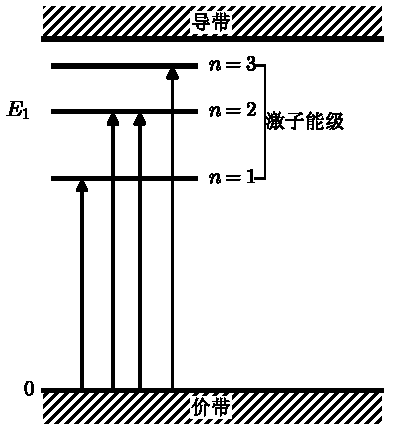
\includegraphics[width=6cm]{fig10-1.pdf}\\{\small 图 10.1\quad 激子能级}
\end{minipage}
\end{center}

以上结果说明：当入射光子能量小于禁带宽度时有一组激子吸收峰出现，吸收峰的位置可根据激子能级公式(10.2.9)确定.对于 $\mathrm{Cu}_{2}\mathrm{O}$ 晶体，其具体计算结果与格洛斯（Gross）等人\textsuperscript{[1]}在低温下测得吸收谱线一致.

式(10.2.9)左边第三项代表激子的平移动能，第二项是形成电子-空穴束缚对时所降低的能量
\begin{equation}
  E_{\mathrm{B}}(n)=-\frac{\overline{M}e^{4}}{2\hbar^{2}\epsilon^{2}n^{2}}
  \equiv\frac{-e^{2}}{2\epsilon n^{2}a_{\mathrm{ex}}}
\end{equation}
其中 $a_{\mathrm{ex}}$ 是基态 $\left(n=1, m=l=0\right)$ 的轨道半径，定义为激子半径.根据氢原子玻尔半径公式 $a_{\mathrm{H}}=\hbar^{2}/m_{\mathrm{e}}e^{2}$（$m_{\mathrm{e}}$ 是真空中电子质量），容易从式(10.2.10)求得激子半径
\begin{equation}
  a_{\mathrm{ex}}=\epsilon\,\frac{\hbar^{2}}{\overline{M}e^{2}}
  =\epsilon\biggl(\frac{m_{\mathrm{e}}}{\overline{M}}\biggr)a_{\mathrm{H}}
\end{equation}
对于瓦尼尔-莫特激子，由于 $a_{\mathrm{ex}}\gg a_{\mathrm{H}}$，必须要求晶体的介电常数 $\epsilon\gg1$，折合质量 $\overline{M}\leqslant m_{\mathrm{e}}$，才能形成大半径的激子.多数的半导体和绝缘晶体满足这一条件，因此瓦尼尔-莫特激子是常见的.根据式(10.2.11)，对于晶格常数较大、介电常数较小的晶体，其激子半径可能比晶格常数小，这时上述理论失效，我们必须考虑晶格的原子结构，从另一角度讨论问题.

\section{夫伦克耳激子}

夫伦克耳认为小激子运动问题实际上是同一原子内电子的激发态从一个原子向另一个原子的转移问题.

设晶体中有 $N$ 个原子，每个原子上有一个电子.原子中电子的基态为 $\phi_{\mathrm{s}}(\boldsymbol{r})$，其能量为 $\mathscr{E}_{\mathrm{s}}$，第一激发态为 $\phi_{\mathrm{p}}(\boldsymbol{r})$，能量是 $\mathscr{E}_{\mathrm{p}}$.因此，原子内电子从s态向p态的激发能为 $\mathscr{E}_{\mathrm{p}}-\mathscr{E}_{\mathrm{s}}$，$N$ 个电子系统的基态，应由 $\phi_{\mathrm{s}}(\boldsymbol{r}_{1}-\boldsymbol{R}_{1}),\cdots,\phi_{\mathrm{s}}(\boldsymbol{r}_{N}-\boldsymbol{R}_{N})$ 的斯莱特行列式组成.为讨论简单起见，在本节中暂时略去电子的自旋和不同格点 $(\boldsymbol{R}_{n}\neq\boldsymbol{R}_{m})$ 间原子波函数的重叠.这样，晶体的基态可写成
\begin{equation}
  \varPhi_{0}(\boldsymbol{r}_{1},\cdots,\boldsymbol{r}_{N})
  =\prod_{m}\phi_{\mathrm{s}}(\boldsymbol{r}_{m}-\boldsymbol{R}_{m})
\end{equation}
假定在第 $n$ 个原子内的电子从s态被激发到p态，则此局域激发态的波函数为
\begin{equation}
  \varPhi_{n}(\boldsymbol{r}_{1},\cdots,\boldsymbol{r}_{N})
  =\phi_{\mathrm{p}}(\boldsymbol{r}_{n}-\boldsymbol{R}_{n})
  \prod_{m(m\neq n)}\phi_{\mathrm{s}}(\boldsymbol{r}_{m}-\boldsymbol{R}_{m})
\end{equation}
$N$ 个原子系统的总哈密顿量由原子的哈密顿量 $h_{n}$ 和原子间互作用 $v_{nm}$ 组成
\begin{equation}
  H=\sum_{n}h_{n}+\sum_{n<m}\sum v_{nm}
\end{equation}
其中 $v_{nm}=e^{2}/|\boldsymbol{r}_{n}-\boldsymbol{r}_{m}|$ 是电子间库仑互作用.

产生如图10.2的局域激发能量为
\begin{equation}
  \mathscr{E}=\langle\varPhi_{n}|H|\varPhi_{n}\rangle
  -\langle\varPhi_{0}|H|\varPhi_{0}\rangle
\end{equation}

\begin{center}
\begin{minipage}{7.5cm}
\centering
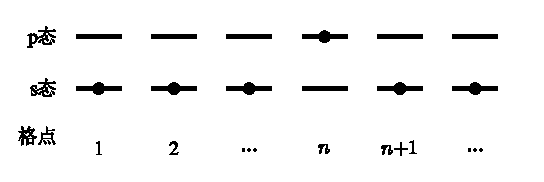
\includegraphics[width=7.5cm]{fig10-2.pdf}\\{\small 图 10.2\quad 局域激发态}
\end{minipage}
\end{center}

在平移对称系统中，此激发能与n无关，它近似等于原子中电子的激发能 $\mathscr{E}_{\mathrm{p}}-\mathscr{E}_{\mathrm{s}}$，说明局域激发可在任何格点产生.另一方面，H的非对角矩阵元为
\begin{equation}
\begin{aligned}
  H_{nm}&=\langle\varPhi_{n}|H|\varPhi_{m}\rangle\\
  &=\iint\mathrm{d}\boldsymbol{r}_{n}\mathrm{d}\boldsymbol{r}_{m}\,
  \phi_{\mathrm{p}}^{*}(\boldsymbol{r}_{n}-\boldsymbol{R}_{n})
  \phi_{\mathrm{s}}^{*}(\boldsymbol{r}_{m}-\boldsymbol{R}_{m})\\
  &\quad\times\frac{e^{2}}{|\boldsymbol{r}_{n}-\boldsymbol{r}_{m}|}
  \phi_{\mathrm{s}}(\boldsymbol{r}_{n}-\boldsymbol{R}_{n})
  \phi_{\mathrm{p}}(\boldsymbol{r}_{m}-\boldsymbol{R}_{m})
\end{aligned}
\end{equation}
{\emergencystretch=1em\relax
$H_{nm}$ 是“电荷分布”$-e\phi_{\mathrm{p}}^{*}(\boldsymbol{r}_{n}-\boldsymbol{R}_{n})\phi_{\mathrm{s}}(\boldsymbol{r}_{n}-\boldsymbol{R}_{n})$ 与 $-e\phi_{\mathrm{s}}^{*}(\boldsymbol{r}_{m}-\boldsymbol{R}_{m})\phi_{\mathrm{p}}(\boldsymbol{r}_{m}-\boldsymbol{R}_{m})$ 之间的库仑互作用，它使n格点原子上的电子激发转移到m格点原子上去，称为激发转移互作用.因此，哈密顿量H的单电子激发本征函数 $\varPsi$ 应当是在各格点上产生局域激发波函数 $\varPhi_{n}$ 的线性组合，与紧束缚近似的能带波函数相似，可将 $\varPsi$ 写为
\begin{equation}
  \varPsi_{\boldsymbol{K}}=\frac{1}{\sqrt{N}}\sum_{n}
  \mathrm{e}^{\mathrm{i}\boldsymbol{K}\cdot\boldsymbol{R}_{n}}\varPhi_{n}
\end{equation}
其中 $\boldsymbol{K}$ 为第一BZ中的波矢，这就是夫伦克耳激子的波函数.夫伦克耳激子的激发能应当由 $\langle\varPsi_{\boldsymbol{K}}|H|\varPsi_{\boldsymbol{K}}\rangle$ $-\langle\varPhi_{0}|H|\varPhi_{0}\rangle$ 决定：\par}
\begin{equation}
\begin{aligned}
  E_{\boldsymbol{K}}&\equiv\langle\varPsi_{\boldsymbol{K}}|H|\varPsi_{\boldsymbol{K}}\rangle
  -\langle\varPhi_{0}|H|\varPhi_{0}\rangle\\
  &=\mathscr{E}+\frac{1}{N}\sum_{m\neq n}\sum\,
  \langle\varPhi_{n}|H|\varPhi_{m}\rangle
  \mathrm{e}^{-\mathrm{i}\boldsymbol{K}\cdot(\boldsymbol{R}_{n}-\boldsymbol{R}_{m})}
\end{aligned}
\end{equation}

由式(10.3.5)可知，$H_{nm}$ 只是 $\boldsymbol{R}_{nm}=\boldsymbol{R}_{n}-\boldsymbol{R}_{m}$ 的函数，记为 $D(\boldsymbol{R}_{nm})$.因此，激子能级可表示为
\begin{equation}
  E_{\boldsymbol{K}}=\mathscr{E}
  +\sum_{\boldsymbol{R}_{nm}}^{\prime}D(\boldsymbol{R}_{nm})
  \mathrm{e}^{-\mathrm{i}\boldsymbol{K}\cdot\boldsymbol{R}_{nm}}
\end{equation}
式(10.3.8)代表夫伦克耳激子的能带公式，一般D很小，是窄带，惰性元素晶体具有这样的激子.例如在原子氪(Kr)组成的晶体中，观测到的激子吸收带很窄，分布在10.17 eV附近，与Kr原子中电子的跃迁能 $9.99$ eV［相当于 $(\mathscr{E}_{\mathrm{p}}-\mathscr{E}_{\mathrm{s}})$］相近，而Kr晶体的禁带宽度 $E_{\mathrm{g}}=11.7$ eV，说明激子能级分布在禁带中，并可用式(10.3.8)确定.

现在具体计算 $H_{nm}$ 的贡献，由式(10.3.5)作变数变换 $(\boldsymbol{r}_{n}-\boldsymbol{R}_{n})=\boldsymbol{r}$，$(\boldsymbol{r}_{m}-\boldsymbol{R}_{m})=\boldsymbol{r}^{\prime}$
\begin{equation}
\begin{aligned}
  H_{nm}&=\iint\mathrm{d}\boldsymbol{r}\mathrm{d}\boldsymbol{r}^{\prime}\,
  \phi_{\mathrm{p}}^{*}(\boldsymbol{r})\phi_{\mathrm{s}}^{*}(\boldsymbol{r}^{\prime})
  \frac{e^{2}}{|\boldsymbol{r}-\boldsymbol{r}^{\prime}-\boldsymbol{R}_{nm}|}
  \phi_{\mathrm{s}}(\boldsymbol{r})\phi_{\mathrm{p}}(\boldsymbol{r}^{\prime})\\
  &=D(\boldsymbol{R}_{nm})
\end{aligned}
\end{equation}
考虑到 $\phi_{\mathrm{s}}$ 和 $\phi_{\mathrm{p}}$ 的空间分布尺度小于原子间距，上式中 $\boldsymbol{\xi}=\boldsymbol{r}-\boldsymbol{r}^{\prime}$ 与 $\boldsymbol{R}_{nm}$ 相比是小量，可作展开：
\begin{equation}
  \frac{1}{|\boldsymbol{\xi}-\boldsymbol{R}_{nm}|}\approx\frac{1}{R_{nm}}
  \biggl[1+\frac{\boldsymbol{\xi}\cdot\boldsymbol{R}_{nm}}{R_{nm}^{2}}
  -\frac{\xi^{2}}{2R_{nm}^{2}}
  +\frac{3}{2}\frac{(\boldsymbol{\xi}\cdot\boldsymbol{R}_{nm})^{2}}{R_{nm}^{4}}
  +\cdots\biggr]
\end{equation}
将式(10.3.10)代入式(10.3.9)，求得
\begin{equation}
  H_{nm}=D(\boldsymbol{R}_{nm})\approx\frac{\mu^{2}}{R_{nm}^{3}}
  -\frac{3(\boldsymbol{\mu}\cdot\boldsymbol{R}_{nm})^{2}}{R_{nm}^{5}}
\end{equation}
其中
\begin{equation}
  \boldsymbol{\mu}\equiv\int\phi_{\mathrm{p}}^{*}(\boldsymbol{r})
  \left(-e\boldsymbol{r}\right)\phi_{\mathrm{s}}(\boldsymbol{r})\mathrm{d}\boldsymbol{r}
\end{equation}
代表偶极矩，式(10.3.11)正好是偶极-偶极相互作用.由此可计算激子能带公式中 $D(\boldsymbol{R}_{nm})$ 的傅里叶变换
\begin{equation}
  D_{\boldsymbol{K}}=\sum_{\boldsymbol{R}_{nm}}^{\prime}D(\boldsymbol{R}_{nm})
  \mathrm{e}^{-\mathrm{i}\boldsymbol{K}\cdot\boldsymbol{R}_{nm}}
\end{equation}
特别是 $D_{\boldsymbol{K}}$ 在 $\boldsymbol{K}=0$ 附近的数值.

设 $Kd\ll1$，这里 $d^{3}=\Omega$，Ω为元胞体积.以某一个原子为中心，作半径为 $R_{\mathrm{c}}$ 的球体，$R_{\mathrm{c}}$ 宏观小、微观大，并满足条件
\begin{equation}
  d\ll R_{\mathrm{c}}\ll K^{-1}
\end{equation}
则在 $R_{\mathrm{c}}$ 球外，求和式(10.3.13)可化为积分，而在 $R_{\mathrm{c}}$ 之内，则取 $\mathrm{e}^{-\mathrm{i}\boldsymbol{K}\cdot\boldsymbol{R}_{nm}}\approx1$.因此，有
\begin{equation}
  D_{\boldsymbol{K}}=\sum_{\boldsymbol{R}_{nm}<R_{\mathrm{c}}}D(\boldsymbol{R}_{nm})+I
\end{equation}
这里 I 是 $R_{\mathrm{c}}$ 球外的积分，求和化积分时利用
$\sum_{\boldsymbol{R}_{nm}}(\cdots)=(1/\Omega)\int(\cdots)\mathrm{d}\boldsymbol{R}$.根据图10.3，取 $\boldsymbol{K}$ 为z轴方向并设 $\theta_{0}$ 代表 $\boldsymbol{K}$ 与偶极矩 $\boldsymbol{\mu}$ 之间的夹角，$\theta$ 为 $\boldsymbol{K}$ 与 $\boldsymbol{R}$ 夹角，$\theta^{\prime}$ 为 $\boldsymbol{R}$ 与 $\boldsymbol{\mu}$ 的夹角，则I表示为积分：
\begin{equation}
\begin{aligned}
  I&=\Omega^{-1}\mu^{2}\int_{R_{\mathrm{c}}}^{\infty}\frac{\mathrm{d}R}{R}
  \int_{0}^{\pi}\mathrm{e}^{-\mathrm{i}KR\cos\theta}\sin\theta\,\mathrm{d}\theta
  \int_{-\pi}^{\pi}\left(1-3\cos^{2}\theta^{\prime}\right)\mathrm{d}\phi\\
  &=-\frac{4\pi}{3}\Omega^{-1}\mu^{2}\left(1-3\cos\theta_{0}^{2}\right)
  +O(K^{2}R_{\mathrm{c}}^{2})
  \qquad\left(Kd\ll1\right)
\end{aligned}
\end{equation}
最后求得，$Kd\ll1$ 时的 $D_{\boldsymbol{K}}$ 值为
\begin{equation}
  D_{\boldsymbol{K}}=\sum_{\boldsymbol{R}_{nm}<R_{\mathrm{c}}}D(\boldsymbol{R}_{nm})
  -\frac{4\pi}{3}\Omega^{-1}
  \Bigl[\mu^{2}-3\frac{(\boldsymbol{\mu}\cdot\boldsymbol{K})^{2}}{K^{2}}\Bigr]
\end{equation}
式(10.3.17)左边第二项在 $\boldsymbol{K}\parallel\boldsymbol{\mu}$ 时（纵向激子态）取 $\left(8\pi/3\right)\Omega^{-1}\mu^{2}$ 值，而 $\boldsymbol{K}\perp\boldsymbol{\mu}$ 时（横向激子态）取 $-\left(4\pi/3\right)\Omega^{-1}\mu^{2}$，两者之差为 $4\pi\Omega^{-1}\mu^{2}$，它代表 $\boldsymbol{K}\to0$ 时纵向和横向激子状态的能级差.纵向和横向激子态间的能级分裂是激子问题中的普遍现象，并非夫伦克耳激子的独特属性.

\begin{center}
\begin{minipage}{5.5cm}
\centering
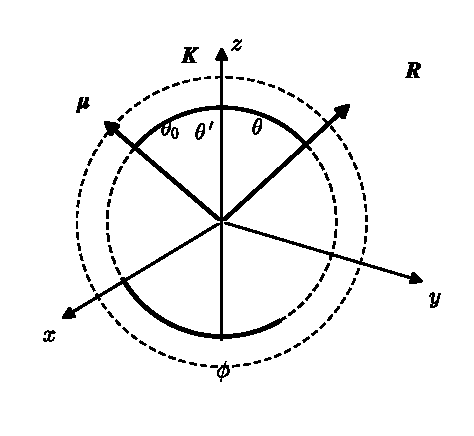
\includegraphics[width=5.5cm]{fig10-3.pdf}\\{\small 图 10.3\quad 积分 I 的计算图}
\end{minipage}
\end{center}

\section{\texorpdfstring{电子-空穴互作用的多体理论\textsuperscript{[2]}}{电子-空穴互作用的多体理论[2]}}

本节用二次量子化方法处理电子-空穴互作用问题，并将在 $a_{\mathrm{ex}}\gg d$ 和 $a_{\mathrm{ex}}\ll d$ 两种极限情况下分别求瓦尼尔-莫特激子和夫伦克耳激子的方程.

设单电子哈密顿量为 $h(\boldsymbol{p},\boldsymbol{r})$，它包括电子的动能和晶格周期场的位能，电子间互作用势能为
\begin{equation}
  v(\boldsymbol{r}-\boldsymbol{r}^{\prime})
  =\frac{e^{2}}{|\boldsymbol{r}-\boldsymbol{r}^{\prime}|}
\end{equation}
多电子系统的哈密顿量在二次量子化表象中写为
\begin{equation}
\begin{aligned}
  H&=\int\mathrm{d}\boldsymbol{r}\,\varPsi^{+}(\boldsymbol{r})h(\boldsymbol{p},\boldsymbol{r})\varPsi(\boldsymbol{r})\\
  &\quad+\frac{1}{2}\iint\mathrm{d}\boldsymbol{r}\mathrm{d}\boldsymbol{r}^{\prime}\,
  \varPsi^{+}(\boldsymbol{r})\varPsi^{+}(\boldsymbol{r}^{\prime})
  v(\boldsymbol{r}-\boldsymbol{r}^{\prime})
  \varPsi(\boldsymbol{r}^{\prime})\varPsi(\boldsymbol{r})
\end{aligned}
\end{equation}
态矢量 $\varPsi(\boldsymbol{r})$ 可分别利用布洛赫函数 $\phi_{\nu\boldsymbol{k}}(\boldsymbol{r})$ 及瓦尼尔函数 $a_{\nu}(\boldsymbol{r}-\boldsymbol{R}_{n})$ 作基函数表示成
\begin{equation}
\begin{aligned}
  \varPsi(\boldsymbol{r})&=\sum_{\nu,\boldsymbol{k}}C_{\nu\boldsymbol{k}}\phi_{\nu\boldsymbol{k}}(\boldsymbol{r})\\
  &=\sum_{\nu,n}C_{\nu n}a_{\nu}(\boldsymbol{r}-\boldsymbol{R}_{n})
\end{aligned}
\end{equation}
$C_{\nu\boldsymbol{k}}$，$C_{\nu\boldsymbol{k}}^{+}$ 代表ν能带中 $\boldsymbol{k}$ 波矢电子的消灭与产生算符，而 $C_{\nu n}$ 和 $C_{\nu n}^{+}$ 则是局域表示中消灭及产生算符，n是格点指标.

利用布洛赫函数与瓦尼尔函数间关系
\begin{equation}
  a_{\nu}(\boldsymbol{r}-\boldsymbol{R}_{n})=(1/\sqrt{N})\sum_{\boldsymbol{k}}
  \mathrm{e}^{-\mathrm{i}\boldsymbol{k}\cdot\boldsymbol{R}_{n}}\phi_{\nu\boldsymbol{k}}(\boldsymbol{r})
\end{equation}
可求得两组算子间关系为
\begin{equation}
  C_{\nu\boldsymbol{k}}=\frac{1}{\sqrt{N}}\sum_{n}
  \mathrm{e}^{-\mathrm{i}\boldsymbol{k}\cdot\boldsymbol{R}_{n}}C_{\nu n}
\end{equation}
算子满足费密子对易律
\begin{equation}
  \bigl[C_{\nu\boldsymbol{k}},C_{\mu\boldsymbol{k}^{\prime}}^{+}\bigr]_{+}
  =\delta_{\nu\mu}\delta_{\boldsymbol{k}\boldsymbol{k}^{\prime}};
  \quad
  \bigl[C_{\nu\boldsymbol{k}},C_{\mu\boldsymbol{k}^{\prime}}\bigr]_{+}
  =\bigl[C_{\nu\boldsymbol{k}}^{+},C_{\mu\boldsymbol{k}^{\prime}}^{+}\bigr]_{+}=0
\end{equation}
\begin{equation}
  \bigl[C_{\nu n},C_{\mu m}^{+}\bigr]_{+}
  =\delta_{\nu\mu}\delta_{nm};
  \quad
  \bigl[C_{\nu n},C_{\mu m}\bigr]_{+}
  =\bigl[C_{\nu n}^{+},C_{\mu m}^{+}\bigr]_{+}=0
\end{equation}
设 $\mu$ 代表绝缘晶体中的满带（价带）指标，ν代表空带（导带）指标，则在单电子近似范围内系统的基态为
\begin{equation}
  |g\rangle=\prod_{\mu^{\prime}\boldsymbol{k}}C_{\mu^{\prime}\boldsymbol{k}}^{+}|0\rangle
\end{equation}
这时 $|0\rangle$ 是真空态，$\mu^{\prime}$ 取所有满带的值.

现在考虑有一个电子从满带的 $(\mu,\boldsymbol{k}^{\prime})$ 态被激发至导带 $(\nu,\boldsymbol{k})$ 态上，形成了 $C_{\nu\boldsymbol{k}}^{+}C_{\mu\boldsymbol{k}^{\prime}}|g\rangle$ 的激发态，这个激发态的总波矢为
\begin{equation}
  \boldsymbol{K}=\boldsymbol{k}-\boldsymbol{k}^{\prime}
\end{equation}
因为在满带 $\mu$ 中失去 $\boldsymbol{k}^{\prime}$ 电子后产生了空穴，其波矢为 $-\boldsymbol{k}^{\prime}$.由于哈密顿量H具有平移对称性，因此总波矢 $\boldsymbol{K}$ 应为量子数，而H的单粒子激发本征函数 $|e\rangle$ 由 $\boldsymbol{K}$ 一定时所有可能的 $(\boldsymbol{k},\boldsymbol{k}^{\prime})$ 激发的线性组合构成
\begin{equation}
  |e\rangle=\sum_{\boldsymbol{k}}f(\boldsymbol{k})
  C_{\nu\boldsymbol{k}}^{+}C_{\mu,\boldsymbol{k}-\boldsymbol{K}}|g\rangle
  \equiv B^{+}|g\rangle
\end{equation}
或利用瓦尼尔表象将上式改写为
\begin{equation}
  |e\rangle=\frac{1}{\sqrt{N}}\sum_{m,l}
  \mathrm{e}^{\mathrm{i}\boldsymbol{K}\cdot\boldsymbol{R}_{m}}F(\boldsymbol{R}_{l})
  C_{\nu,m+l}^{+}C_{\mu m}|g\rangle\equiv B^{+}|g\rangle
\end{equation}
其中
\begin{equation}
\left.
\begin{aligned}
  F(\boldsymbol{R}_{l})&=\frac{1}{\sqrt{N}}\sum_{\boldsymbol{k}}f(\boldsymbol{k})
  \mathrm{e}^{\mathrm{i}\boldsymbol{k}\cdot\boldsymbol{R}_{l}}\\
  f(\boldsymbol{k})&=\frac{1}{\sqrt{N}}\sum_{l}F(\boldsymbol{R}_{l})
  \mathrm{e}^{-\mathrm{i}\boldsymbol{k}\cdot\boldsymbol{R}_{l}}
\end{aligned}\right\}
\end{equation}
$f$ 与 $F$ 的归一条件为
\begin{equation}
  \sum_{\boldsymbol{k}}|f(\boldsymbol{k})|^{2}
  =\sum_{l}|F(\boldsymbol{R}_{l})|^{2}=1
\end{equation}
为简单起见，在导出式(10.4.11)时，我们只限于考虑系统中激发了电子和空穴的价带 $\mu$ 和导带ν，而略去其它能带的影响.

式(10.4.10)和(10.4.11)中 $f(\boldsymbol{k})$ 及 $F(\boldsymbol{R}_{l})$ 是二体运动的概率振幅.例如，$F(\boldsymbol{R}_{l})$ 代表导带ν中有一个电子，价带 $\mu$ 中有一个空穴的相对波函数，$\boldsymbol{R}_{l}$ 是电子-空穴的相对坐标，$\boldsymbol{K}$ 代表电子-空穴对平移运动的波矢，如果能求得 $F(\boldsymbol{R}_{l})$ 或 $f(\boldsymbol{k})$ 所满足的运动方程，那么N粒子问题就简化为二体问题了.下面，我们首先给出哈特利-福克近似下的二体运动方程，然后分别讨论大激子与小激子的极限情况.

\subsection*{1. $f(\boldsymbol{k})$和$F(\boldsymbol{R}_{l})$的运动方程}

我们的目的是求激发态 $|e\rangle$ 和激发能
\begin{equation}
  E=E_{e}-E_{0}
\end{equation}
其中 $E_{0}$ 是基态 $|g\rangle$ 的能量，$E_{e}$ 是激发态 $|e\rangle$ 的能量，它们分别满足本征方程
\begin{equation}
  0=\left(H-E_{0}\right)|g\rangle
\end{equation}
和
\begin{equation}
  0=\left(H-E_{e}\right)|e\rangle
\end{equation}
利用式(10.4.10)引入算符 $B^{+}$，可将 $|e\rangle$ 的本征方程改写为
\begin{equation}
\begin{aligned}
  0&=\left(H-E_{e}\right)|e\rangle\\
  &=\left(HB^{+}-E_{e}B^{+}\right)|g\rangle\\
  &=\left(\left[H,B^{+}\right]+B^{+}H-E_{e}B^{+}\right)|g\rangle
\end{aligned}
\end{equation}
利用式(10.4.14)和(10.4.15)，得到算符 $B^{+}$ 的方程
\begin{equation}
  \left[H,B^{+}\right]|g\rangle=EB^{+}|g\rangle
\end{equation}
E 为激发能.将式(10.4.10)所给出的 $B^{+}$ 代入上式，并左乘 $\langle g|C_{\mu\boldsymbol{k}^{\prime}-\boldsymbol{K}}^{+}C_{\nu\boldsymbol{k}^{\prime}}$ 可求得 $f(\boldsymbol{k})$ 的运动方程
\begin{equation}
  \sum_{\boldsymbol{k}}H_{\boldsymbol{k}^{\prime}\boldsymbol{k}}f(\boldsymbol{k})
  =Ef(\boldsymbol{k}^{\prime})
\end{equation}
这里有效哈密顿量 $H_{\boldsymbol{k}^{\prime}\boldsymbol{k}}$ 定义为
\begin{equation}
  H_{\boldsymbol{k}^{\prime}\boldsymbol{k}}\equiv\langle g|
  C_{\mu,\boldsymbol{k}^{\prime}-\boldsymbol{K}}^{+}C_{\nu\boldsymbol{k}^{\prime}}
  \left[H,C_{\nu\boldsymbol{k}}^{+}C_{\mu,\boldsymbol{k}-\boldsymbol{K}}\right]|g\rangle
\end{equation}
利用对易关系式(10.4.6)，经直接计算可以求得哈特利-福克近似的结果为
\begin{equation}
\begin{aligned}
  H_{\boldsymbol{k}^{\prime}\boldsymbol{k}}
  &=\delta_{\boldsymbol{k}^{\prime}\boldsymbol{k}}\{\mathscr{E}_{\nu}(\boldsymbol{k})
  -\mathscr{E}_{\mu}(\boldsymbol{k}-\boldsymbol{K})\}\\
  &\quad-\langle\nu,\boldsymbol{k}^{\prime};\mu,(\boldsymbol{k}-\boldsymbol{K})|v|
  \nu,\boldsymbol{k};\mu,(\boldsymbol{k}^{\prime}-\boldsymbol{K})\rangle\\
  &\quad+\langle\nu,\boldsymbol{k}^{\prime};\mu,(\boldsymbol{k}-\boldsymbol{K})|v|
  \mu,(\boldsymbol{k}^{\prime}-\boldsymbol{K});\nu,k\rangle
\end{aligned}
\end{equation}
这里
\begin{equation}
\begin{aligned}
  &\langle\lambda_{1},\boldsymbol{k}_{1};\lambda_{2},\boldsymbol{k}_{2}|v|
  \lambda_{3},\boldsymbol{k}_{3};\lambda_{4},\boldsymbol{k}_{4}\rangle\\
  &\equiv\iint\mathrm{d}\boldsymbol{r}\mathrm{d}\boldsymbol{r}^{\prime}\,
  \phi_{\lambda_{1}\boldsymbol{k}_{1}}^{*}(\boldsymbol{r})
  \phi_{\lambda_{2}\boldsymbol{k}_{2}}^{*}(\boldsymbol{r}^{\prime})
  v(\boldsymbol{r}-\boldsymbol{r}^{\prime})
  \phi_{\lambda_{3}\boldsymbol{k}_{3}}(\boldsymbol{r})
  \phi_{\lambda_{4}\boldsymbol{k}_{4}}(\boldsymbol{r}^{\prime})
\end{aligned}
\end{equation}
显然，式(10.4.21)右边第三项代表库仑势作用，第四项为交换作用.应当注意到式(10.4.21)中第三、四项与电子-电子互作用情况相差负号，这是由于激子问题涉及电子与空穴相互作用，而空穴带正电的缘故.$\mathscr{E}_{\nu}(\boldsymbol{k})$ 和 $\mathscr{E}_{\mu}(\boldsymbol{k}-\boldsymbol{K})$ 为导带及满带中电子在哈特利-福克近似下的能量，它满足HF方程
\begin{equation}
\begin{aligned}
  &h(\boldsymbol{p},\boldsymbol{r})\phi_{\lambda\boldsymbol{k}}(\boldsymbol{r})
  +\sum_{\mu^{\prime},\boldsymbol{k}^{\prime}}\int\mathrm{d}\boldsymbol{r}^{\prime}\,
  v(\boldsymbol{r}-\boldsymbol{r}^{\prime})\phi_{\mu^{\prime}\boldsymbol{k}^{\prime}}(\boldsymbol{r}^{\prime})
  \times\\
  &\qquad\left[\phi_{\mu^{\prime}\boldsymbol{k}^{\prime}}(\boldsymbol{r}^{\prime})\phi_{\lambda\boldsymbol{k}}(\boldsymbol{r})
  -\phi_{\mu^{\prime}\boldsymbol{k}^{\prime}}(\boldsymbol{r})\phi_{\lambda\boldsymbol{k}}(\boldsymbol{r}^{\prime})\right]\\
  &\qquad=\mathscr{E}_{\lambda}(\boldsymbol{k})\phi_{\lambda\boldsymbol{k}}(\boldsymbol{r})
\end{aligned}
\end{equation}
利用式(10.4.12)将 $\boldsymbol{k}$ 表象中 $f(\boldsymbol{k})$ 的运动方程(10.4.19)变换到 $\boldsymbol{R}$ 表象，从而求得 $F(\boldsymbol{R})$ 的运动方程
\begin{equation}
  \sum_{l^{\prime}}H_{l^{\prime}l}F(\boldsymbol{R}_{l^{\prime}})=EF(\boldsymbol{R}_{l})
\end{equation}
这里
\begin{equation}
  H_{l^{\prime}l}=\frac{1}{N}\sum_{\boldsymbol{k},\boldsymbol{k}^{\prime}}
  \mathrm{e}^{\mathrm{i}\boldsymbol{k}^{\prime}\cdot\boldsymbol{R}_{l}}H_{\boldsymbol{k}^{\prime}\boldsymbol{k}}
  \mathrm{e}^{-\mathrm{i}\boldsymbol{k}\cdot\boldsymbol{R}_{l^{\prime}}}
\end{equation}
其中 $\boldsymbol{R}_{l}$ 是电子-空穴的相对坐标.将式(10.4.21)代入式(10.4.25)
\begin{equation}
\begin{aligned}
  H_{l^{\prime}l}&=\frac{1}{N}\sum_{\boldsymbol{k}^{\prime}}
  \mathscr{E}_{\nu}(\boldsymbol{k}^{\prime})
  \mathrm{e}^{\mathrm{i}\boldsymbol{k}^{\prime}\cdot(\boldsymbol{R}_{l}-\boldsymbol{R}_{l^{\prime}})}
  -\frac{1}{N}\sum_{\boldsymbol{k}}\mathscr{E}_{\mu}(\boldsymbol{k}-\boldsymbol{K})
  \mathrm{e}^{\mathrm{i}\boldsymbol{k}\cdot(\boldsymbol{R}_{l}-\boldsymbol{R}_{l^{\prime}})}\\
  &\quad-\frac{1}{N}\sum_{\boldsymbol{k},\boldsymbol{k}^{\prime}}
  \mathrm{e}^{\mathrm{i}\boldsymbol{k}^{\prime}\cdot\boldsymbol{R}_{l}}
  \langle\mathrm{I}\rangle
  \mathrm{e}^{-\mathrm{i}\boldsymbol{k}\cdot\boldsymbol{R}_{l^{\prime}}}
  +\frac{1}{N}\sum_{\boldsymbol{k},\boldsymbol{k}^{\prime}}
  \mathrm{e}^{\mathrm{i}\boldsymbol{k}^{\prime}\cdot\boldsymbol{R}_{l^{\prime}}}
  \langle\mathrm{II}\rangle
  \mathrm{e}^{-\mathrm{i}\boldsymbol{k}\cdot\boldsymbol{R}_{l^{\prime}}}
\end{aligned}
\end{equation}
这里 $\langle\mathrm{I}\rangle$ 代表式(10.4.21)中库仑项，$\langle\mathrm{II}\rangle$ 是交换作用项.
\begin{equation}
\begin{aligned}
  \langle\mathrm{I}\rangle&\equiv\langle\nu,\boldsymbol{k}^{\prime};
  \mu,(\boldsymbol{k}-\boldsymbol{K})|v|\nu,\boldsymbol{k};
  \mu,(\boldsymbol{k}^{\prime}-\boldsymbol{K})\rangle\\
  &=\iint\mathrm{d}\boldsymbol{r}\mathrm{d}\boldsymbol{r}^{\prime}\,
  \phi_{\nu\boldsymbol{k}^{\prime}}^{*}(\boldsymbol{r})
  \phi_{\mu(\boldsymbol{k}-\boldsymbol{K})}^{*}(\boldsymbol{r}^{\prime})
  v(\boldsymbol{r}-\boldsymbol{r}^{\prime})
  \phi_{\nu\boldsymbol{k}}(\boldsymbol{r})
  \phi_{\mu(\boldsymbol{k}^{\prime}-\boldsymbol{K})}(\boldsymbol{r}^{\prime})\\
  &=\frac{1}{N^{2}}\sum_{\boldsymbol{R}_{1}\cdots\boldsymbol{R}_{4}}
  \exp\bigl\{-\mathrm{i}[\boldsymbol{k}^{\prime}\cdot\boldsymbol{R}_{1}
  +(\boldsymbol{k}-\boldsymbol{K})\cdot\boldsymbol{R}_{2}
  -\boldsymbol{k}\cdot\boldsymbol{R}_{3}
  -(\boldsymbol{k}^{\prime}-\boldsymbol{K})\cdot\boldsymbol{R}_{4}]\bigr\}\\
  &\qquad\times\iint\mathrm{d}\boldsymbol{r}\mathrm{d}\boldsymbol{r}^{\prime}\,
  \boldsymbol{a}_{\nu}^{*}(\boldsymbol{r}-\boldsymbol{R}_{1})
  \boldsymbol{a}_{\mu}^{*}(\boldsymbol{r}^{\prime}-\boldsymbol{R}_{2})
  v(\boldsymbol{r}-\boldsymbol{r}^{\prime})
  \boldsymbol{a}_{\nu}(\boldsymbol{r}-\boldsymbol{R}_{3})
  \boldsymbol{a}_{\mu}(\boldsymbol{r}^{\prime}-\boldsymbol{R}_{4})\\
  &\approx\frac{1}{N^{2}}\sum_{\boldsymbol{R}_{1},\boldsymbol{R}_{2}}
  \exp\bigl\{-\mathrm{i}(\boldsymbol{k}^{\prime}-\boldsymbol{k})
  \cdot(\boldsymbol{R}_{1}-\boldsymbol{R}_{2})\bigr\}\\
  &\qquad\times\iint\mathrm{d}\boldsymbol{r}\mathrm{d}\boldsymbol{r}^{\prime}\,
  \boldsymbol{a}_{\nu}^{*}(\boldsymbol{r}-\boldsymbol{R}_{1})
  \boldsymbol{a}_{\mu}^{*}(\boldsymbol{r}^{\prime}-\boldsymbol{R}_{2})
  v(\boldsymbol{r}-\boldsymbol{r}^{\prime})
  \boldsymbol{a}_{\nu}(\boldsymbol{r}-\boldsymbol{R}_{1})
  \boldsymbol{a}_{\mu}(\boldsymbol{r}^{\prime}-\boldsymbol{R}_{2})\\
  &\equiv\frac{1}{N}\sum_{\boldsymbol{R}_{12}}
  \mathrm{e}^{-\mathrm{i}(\boldsymbol{k}^{\prime}-\boldsymbol{k})\cdot\boldsymbol{R}_{12}}
  V(\boldsymbol{R}_{12})
  \qquad(\boldsymbol{R}_{12}=\boldsymbol{R}_{1}-\boldsymbol{R}_{2})
\end{aligned}
\end{equation}
上式中利用了瓦尼尔函数 $\boldsymbol{a}_{\lambda}(\boldsymbol{r}-\boldsymbol{R}_{n})$ 的局域特性，认为瓦尼尔函数与原子轨道函数相似，是局限于 $\boldsymbol{R}_{n}$ 格点周围的函数.这时可近似取 $\boldsymbol{R}_{1}=\boldsymbol{R}_{3}$ 和 $\boldsymbol{R}_{2}=\boldsymbol{R}_{4}$，并得到式(10.4.27)的第四个等式.

类似的，用瓦尼尔函数表示 $\langle\mathrm{II}\rangle$，可求得如下结果：
\begin{equation}
\begin{aligned}
  \langle\mathrm{II}\rangle&\equiv\langle\nu,\boldsymbol{k}^{\prime};
  \mu,(\boldsymbol{k}-\boldsymbol{K})|v|\mu,(\boldsymbol{k}^{\prime}-\boldsymbol{K});
  \nu,k\rangle\\
  &=\frac{1}{N^{2}}\sum_{\boldsymbol{R}_{1}\cdots\boldsymbol{R}_{4}}
  \exp\bigl\{-\mathrm{i}[\boldsymbol{k}^{\prime}\cdot\boldsymbol{R}_{1}
  +(\boldsymbol{k}-\boldsymbol{K})\cdot\boldsymbol{R}_{2}\\
  &\qquad-(\boldsymbol{k}^{\prime}-\boldsymbol{K})\cdot\boldsymbol{R}_{3}
  -\boldsymbol{k}\cdot\boldsymbol{R}_{4}]\bigr\}
  \times\iint\mathrm{d}\boldsymbol{r}\mathrm{d}\boldsymbol{r}^{\prime}\,
  \boldsymbol{a}_{\nu}^{*}(\boldsymbol{r}-\boldsymbol{R}_{1})
  \boldsymbol{a}_{\mu}^{*}(\boldsymbol{r}^{\prime}-\boldsymbol{R}_{2})\\
  &\qquad\times v(\boldsymbol{r}-\boldsymbol{r}^{\prime})
  \boldsymbol{a}_{\mu}(\boldsymbol{r}-\boldsymbol{R}_{3})
  \boldsymbol{a}_{\nu}(\boldsymbol{r}^{\prime}-\boldsymbol{R}_{4})\\
  &\approx\frac{1}{N^{2}}\sum_{\boldsymbol{R}_{1},\boldsymbol{R}_{2}}
  \exp\bigl\{-\mathrm{i}\boldsymbol{K}\cdot(\boldsymbol{R}_{1}-\boldsymbol{R}_{2})\bigr\}\\
  &\qquad\times\iint\mathrm{d}\boldsymbol{r}\mathrm{d}\boldsymbol{r}^{\prime}\,
  \boldsymbol{a}_{\nu}^{*}(\boldsymbol{r}-\boldsymbol{R}_{1})
  \boldsymbol{a}_{\mu}^{*}(\boldsymbol{r}^{\prime}-\boldsymbol{R}_{2})
  v(\boldsymbol{r}-\boldsymbol{r}^{\prime})
  \boldsymbol{a}_{\mu}(\boldsymbol{r}-\boldsymbol{R}_{1})
  \boldsymbol{a}_{\nu}(\boldsymbol{r}^{\prime}-\boldsymbol{R}_{2})\\
  &\equiv\frac{1}{N}\sum_{\boldsymbol{R}_{12}}
  \mathrm{e}^{-\mathrm{i}\boldsymbol{K}\cdot\boldsymbol{R}_{12}}W(\boldsymbol{R}_{12})
\end{aligned}
\end{equation}
这样，式(10.4.26)右边第三、四项为
\begin{equation}
\left.
\begin{aligned}
  \frac{1}{N}\sum_{\boldsymbol{k},\boldsymbol{k}^{\prime}}
  \mathrm{e}^{\mathrm{i}\boldsymbol{k}^{\prime}\cdot\boldsymbol{R}_{l}}
  \langle\mathrm{I}\rangle
  \mathrm{e}^{-\mathrm{i}\boldsymbol{k}\cdot\boldsymbol{R}_{l^{\prime}}}
  &=\delta_{ll^{\prime}}V(\boldsymbol{R}_{l})\\
  \frac{1}{N}\sum_{\boldsymbol{k},\boldsymbol{k}^{\prime}}
  \mathrm{e}^{\mathrm{i}\boldsymbol{k}^{\prime}\cdot\boldsymbol{R}_{l}}
  \langle\mathrm{II}\rangle
  \mathrm{e}^{-\mathrm{i}\boldsymbol{k}\cdot\boldsymbol{R}_{l^{\prime}}}
  &=\delta_{l0}\delta_{l^{\prime}0}W_{\boldsymbol{K}}
\end{aligned}\right\}
\end{equation}
其中
\begin{equation*}
  W_{\boldsymbol{K}}=\sum_{m}\mathrm{e}^{-\mathrm{i}\boldsymbol{K}\cdot\boldsymbol{R}_{m}}W(\boldsymbol{R}_{m})
\end{equation*}
根据式(10.4.27)与(10.4.28)，$V(\boldsymbol{R}_{l})$ 和 $W(\boldsymbol{R}_{m})$ 定义为
\begin{equation}
  V(\boldsymbol{R}_{l})\equiv\iint\mathrm{d}\boldsymbol{r}\mathrm{d}\boldsymbol{r}^{\prime}\,
  \boldsymbol{a}_{\nu}^{*}(\boldsymbol{r}-\boldsymbol{R}_{l})
  \boldsymbol{a}_{\mu}^{*}(\boldsymbol{r}^{\prime})
  v(\boldsymbol{r}-\boldsymbol{r}^{\prime})
  \boldsymbol{a}_{\nu}(\boldsymbol{r}-\boldsymbol{R}_{l})
  \boldsymbol{a}_{\mu}(\boldsymbol{r}^{\prime})
\end{equation}
\begin{equation}
  W(\boldsymbol{R}_{m})\equiv\int\mathrm{d}\boldsymbol{r}\mathrm{d}\boldsymbol{r}^{\prime}\,
  \boldsymbol{a}_{\nu}^{*}(\boldsymbol{r}-\boldsymbol{R}_{m})
  \boldsymbol{a}_{\mu}^{*}(\boldsymbol{r}^{\prime})
  v(\boldsymbol{r}-\boldsymbol{r}^{\prime})
  \boldsymbol{a}_{\mu}(\boldsymbol{r}-\boldsymbol{R}_{m})
  \boldsymbol{a}_{\nu}(\boldsymbol{r}^{\prime})
\end{equation}
式(10.4.26)右边第一项可定义为 $E_{\nu}(\boldsymbol{R}_{l}-\boldsymbol{R}_{l^{\prime}})$
\begin{equation}
  E_{\nu}(\boldsymbol{R}_{l}-\boldsymbol{R}_{l^{\prime}})\equiv\frac{1}{N}
  \sum_{\boldsymbol{k}}\mathscr{E}_{\nu}(\boldsymbol{k})
  \mathrm{e}^{\mathrm{i}\boldsymbol{k}\cdot(\boldsymbol{R}_{l}-\boldsymbol{R}_{l^{\prime}})}
\end{equation}
其逆变换是
\begin{equation}
  \mathscr{E}_{\nu}(\boldsymbol{k})=\sum_{m}E_{\nu}(\boldsymbol{R}_{m})
  \mathrm{e}^{-\mathrm{i}\boldsymbol{k}\cdot\boldsymbol{R}_{m}}
\end{equation}
由于 $E_{\nu}(\boldsymbol{R}_{l}-\boldsymbol{R}_{l^{\prime}})$ 项在方程式(10.4.24)中是作用于函数F上的，我们可以利用第八章§8讨论有效哈密顿量时的技巧作下列简化：
\begin{equation}
\begin{aligned}
  \sum_{l^{\prime}}E_{\nu}(\boldsymbol{R}_{l}-\boldsymbol{R}_{l^{\prime}})F(\boldsymbol{R}_{l^{\prime}})
  &=\sum_{m}E_{\nu}(\boldsymbol{R}_{m})F(\boldsymbol{R}_{l}-\boldsymbol{R}_{m})\\
  &=\sum_{m}E_{\nu}(\boldsymbol{R}_{m})\sum_{p=0}^{\infty}\frac{1}{p!}
  (-\boldsymbol{R}_{m}\cdot\nabla_{l})^{p}F(\boldsymbol{R}_{l})\\
  &=\sum_{m}E_{\nu}(\boldsymbol{R}_{m})
  \exp[-\boldsymbol{R}_{m}\cdot\nabla_{l}]F(\boldsymbol{R}_{l})\\
  &=\mathscr{E}_{\nu}(-\mathrm{i}\nabla_{l})F(\boldsymbol{R}_{l})\\
  &=\sum_{l^{\prime}}\mathscr{E}_{\nu}(-\mathrm{i}\nabla_{l})\delta_{ll^{\prime}}F(\boldsymbol{R}_{l^{\prime}})
\end{aligned}
\end{equation}
这时式(10.4.26)右边第二项可写成
\begin{equation}
\begin{aligned}
  \frac{1}{N}\sum_{\boldsymbol{k}}\mathscr{E}_{\mu}(\boldsymbol{k}-\boldsymbol{K})
  \mathrm{e}^{\mathrm{i}\boldsymbol{k}\cdot(\boldsymbol{R}_{l}-\boldsymbol{R}_{l^{\prime}})}
  &=\mathrm{e}^{\mathrm{i}\boldsymbol{K}\cdot(\boldsymbol{R}_{l}-\boldsymbol{R}_{l^{\prime}})}
  \frac{1}{N}\sum_{\boldsymbol{k}}\mathscr{E}_{\mu}(\boldsymbol{k})
  \mathrm{e}^{\mathrm{i}\boldsymbol{k}\cdot(\boldsymbol{R}_{l}-\boldsymbol{R}_{l^{\prime}})}\\
  &=\mathrm{e}^{\mathrm{i}\boldsymbol{K}\cdot(\boldsymbol{R}_{l}-\boldsymbol{R}_{l^{\prime}})}
  E(\boldsymbol{R}_{l}-\boldsymbol{R}_{l^{\prime}})
\end{aligned}
\end{equation}
类似于式(10.4.34)的作法，求得这一项在F方程(10.4.24)中的贡献为
\begin{equation}
\begin{aligned}
  &\sum_{l^{\prime}}\mathrm{e}^{\mathrm{i}\boldsymbol{K}\cdot(\boldsymbol{R}_{l}-\boldsymbol{R}_{l^{\prime}})}
  E_{\mu}(\boldsymbol{R}_{l}-\boldsymbol{R}_{l^{\prime}})F(\boldsymbol{R}_{l^{\prime}})\\
  &\quad=\sum_{m}\mathrm{e}^{\mathrm{i}\boldsymbol{K}\cdot\boldsymbol{R}_{m}}
  E_{\mu}(\boldsymbol{R}_{m})F(\boldsymbol{R}_{l}-\boldsymbol{R}_{m})\\
  &\quad=\sum_{m}E_{\mu}(\boldsymbol{R}_{m})
  \exp[\boldsymbol{R}_{m}\cdot(-\nabla_{l}+\mathrm{i}\boldsymbol{K})]F(\boldsymbol{R}_{l})\\
  &\quad=\mathscr{E}_{\mu}(-\mathrm{i}\nabla_{l}-\boldsymbol{K})F(\boldsymbol{R}_{l})\\
  &\quad=\sum_{l^{\prime}}\mathscr{E}_{\mu}(-\mathrm{i}\nabla_{l}-\boldsymbol{K})\delta_{ll^{\prime}}F(\boldsymbol{R}_{l^{\prime}})
\end{aligned}
\end{equation}
根据式(10.4.26)和(10.4.29)—(10.4.36)，可将电子-空穴对激发的有效哈密顿量，写成下列简单形式：
\begin{equation}
  H_{ll^{\prime}}=\{\mathscr{E}_{\nu}(-\mathrm{i}\nabla_{l})
  -\mathscr{E}_{\mu}(-\mathrm{i}\nabla_{l}-\boldsymbol{K})-V(\boldsymbol{R}_{l})\}\delta_{ll^{\prime}}
  +\delta_{l0}\delta_{l^{\prime}0}W_{\boldsymbol{K}}
\end{equation}
将上式代入F的运动方程(10.4.24)，可统一处理大激子与小激子问题.我们将证明：在激子半径比晶格常数大的极限情况下，可导出瓦尼尔-莫特激子方程(10.2.5).在相反极限下，则求出夫伦克耳激子的能带公式(10.3.8).

\subsection*{2. 瓦尼尔-莫特激子}

当价带 $\mu$ 中空穴与导带ν中电子的相对距离 $\boldsymbol{R}$ 比较大时，可以忽略 $H_{ll^{\prime}}$ 中交换项 $W_{\boldsymbol{K}}$ 的贡献，因为它是短程作用.$H_{ll^{\prime}}$ 中重要的是库仑项 $V(\boldsymbol{R})$，它是长程作用.根据式(10.4.30)，考虑到瓦尼尔函数 $|\boldsymbol{a}_{\nu}(\boldsymbol{r}-\boldsymbol{R})|^{2}$ 是集中分布在 $\boldsymbol{R}$ 附近的局域函数，可将库仑项写成下列近似式：
\begin{equation}
\begin{aligned}
  V(\boldsymbol{R})&=\iint\mathrm{d}\boldsymbol{r}\mathrm{d}\boldsymbol{r}^{\prime}\,
  |\boldsymbol{a}_{\nu}(\boldsymbol{r}-\boldsymbol{R})|^{2}
  |\boldsymbol{a}_{\mu}(\boldsymbol{r}^{\prime})|^{2}
  \cdot\frac{e^{2}}{|\boldsymbol{r}-\boldsymbol{r}^{\prime}|}\\
  &\approx\frac{e^{2}}{R}
\end{aligned}
\end{equation}
这时激子运动方程(10.4.24)为
\begin{equation}
  \biggl\{\mathscr{E}_{\nu}(-\mathrm{i}\nabla_{R})
  -\mathscr{E}_{\mu}(-\mathrm{i}\nabla_{R}-\boldsymbol{K})
  -\frac{e^{2}}{R}\biggr\}F(\boldsymbol{R})=EF(\boldsymbol{R})
\end{equation}
式(10.4.39)实际上是导带中有一个能量为 $\mathscr{E}_{\nu}(\boldsymbol{k})$ 的电子，价带中有能量为 $-\mathscr{E}_{\mu}(\boldsymbol{k}-\boldsymbol{K})$ 的空穴，电子与空穴之间库仑作用为 $-e^{2}/R$ 的二体运动方程，$\{\cdots\}$ 代表有效哈密顿量.利用有效质量近似
\begin{equation}
\left.
\begin{aligned}
  \mathscr{E}_{\nu}(\boldsymbol{k})&=E_{\mathrm{g}}+\frac{\hbar^{2}k^{2}}{2m_{\mathrm{e}}^{*}}\\
  \mathscr{E}_{\mu}(\boldsymbol{k})&=-\frac{\hbar^{2}k^{2}}{2m_{\mathrm{h}}^{*}}
\end{aligned}\right\}
\end{equation}
不难导出§2中瓦尼尔-莫特激子方程.为此，先对式(10.4.39)作变换
\begin{equation}
  F(\boldsymbol{R})=\widetilde{F}(\boldsymbol{R})
  \exp\biggl\{\frac{\mathrm{i}}{2}\boldsymbol{K}\cdot\boldsymbol{R}\biggr\}
\end{equation}
使方程写成下列对称形式：
\begin{equation}
  \biggl\{\mathscr{E}_{\nu}\biggl(-\mathrm{i}\nabla_{R}
  +\frac{\boldsymbol{K}}{2}\biggr)
  -\mathscr{E}_{\mu}\biggl(-\mathrm{i}\nabla_{R}
  -\frac{\boldsymbol{K}}{2}\biggr)
  -\frac{e^{2}}{R}\biggr\}\widetilde{F}(\boldsymbol{R})=E\widetilde{F}(\boldsymbol{R})
\end{equation}
再利用 $\mathscr{E}_{\nu}$ 和 $\mathscr{E}_{\mu}$ 的有效质量公式(10.4.40)，得到
\begin{equation}
\begin{aligned}
  &\Bigl[-\frac{\hbar^{2}}{2\overline{M}}\nabla_{R}^{2}
  -\frac{e^{2}}{R}
  -\frac{\hbar^{2}}{2\mathrm{i}}\biggl(\frac{1}{m_{\mathrm{h}}^{*}}
  -\frac{1}{m_{\mathrm{e}}^{*}}\biggr)\boldsymbol{K}\cdot\nabla_{R}\Bigr]\widetilde{F}(\boldsymbol{R})\\
  &\qquad=\biggl(E-E_{\mathrm{g}}-\frac{\hbar^{2}K^{2}}{8\overline{M}}\biggr)\widetilde{F}(\boldsymbol{R})
\end{aligned}
\end{equation}
其中折合质量 $\left(\overline{M}\right)^{-1}
=\left(m_{\mathrm{e}}^{*}\right)^{-1}
+\left(m_{\mathrm{h}}^{*}\right)^{-1}$.对上式再作变换
\begin{equation}
  \widetilde{F}(\boldsymbol{R})=f(\boldsymbol{R})\exp
  \biggl\{\frac{\mathrm{i}}{2}\frac{m_{\mathrm{e}}^{*}-m_{\mathrm{h}}^{*}}
  {m_{\mathrm{e}}^{*}+m_{\mathrm{h}}^{*}}\boldsymbol{K}\cdot\boldsymbol{R}\biggr\}
\end{equation}
可消去式(10.4.43)中的 $\boldsymbol{K}\cdot\nabla$ 项，最后得到瓦尼尔-莫特激子的相对运动方程
\begin{equation}
  \Biggl(-\frac{\hbar^{2}}{2\overline{M}}\nabla_{R}^{2}
  -\frac{e^{2}}{R}\Biggr)f(\boldsymbol{R})
  =\Biggl(E-E_{\mathrm{g}}-\frac{\hbar^{2}K^{2}}{2M}\Biggr)f(\boldsymbol{R})
\end{equation}
这里 $E_{\mathrm{g}}$ 为禁带宽度，$\boldsymbol{K}$ 为激子平移运动波矢，$M=m_{\mathrm{e}}^{*}+m_{\mathrm{h}}^{*}$ 是激子的平移质量，$\overline{M}$ 代表折合质量.式(10.4.45)与瓦尼尔-莫特激子方程(10.2.5)相同，唯一的差别是这里的库仑项中少了屏蔽常数 $1/\epsilon$，因为在推导式(10.4.45)时，我们只考虑了一个电子-空穴对激发，从而忽略了晶体介电极化对电子和空穴互作用的影响.作为一个严格的多体理论，还应当计及更多电子-空穴对激发的影响，具体可依照第四章中无规相近似法.最后求得的方程中将出现屏蔽势 $-e^{2}/\epsilon R$，与§2中从唯象模型导出的激子方程完全一致.由于其基本精神与以上推导相同，而且计算较繁，这里不再介绍.

\subsection*{3. 夫伦克耳激子}

先根据式(10.4.37)和(10.4.24)，写出激发能的一般公式.因为F的方程为
\begin{equation}
  \bigl\{\mathscr{E}_{\nu}(-\mathrm{i}\nabla_{l})
  -\mathscr{E}_{\mu}(-\mathrm{i}\nabla_{l}-\boldsymbol{K})
  -V(\boldsymbol{R}_{l})\bigr\}F(\boldsymbol{R}_{l})
  +W_{\boldsymbol{K}}F(0)=EF(\boldsymbol{R}_{l})
\end{equation}
上式乘 $F^{*}(\boldsymbol{R}_{l})$ 对l求和，并利用归一条件
$\sum_{l}|F(\boldsymbol{R}_{l})|^{2}=1$ 和式(10.4.34)及式(10.4.36)，求出激发能公式
\begin{equation}
\begin{aligned}
  E&=\sum_{l,l^{\prime}}F^{*}(\boldsymbol{R}_{l})H_{ll^{\prime}}F(\boldsymbol{R}_{l^{\prime}})\\
  &=\sum_{l,l^{\prime}}\bigl\{E_{\nu}(\boldsymbol{R}_{l}-\boldsymbol{R}_{l^{\prime}})
  -\mathrm{e}^{\mathrm{i}\boldsymbol{K}\cdot(\boldsymbol{R}_{l}-\boldsymbol{R}_{l^{\prime}})}
  E_{\mu}(\boldsymbol{R}_{l}-\boldsymbol{R}_{l^{\prime}})\bigr\}\\
  &\quad\times F^{*}(\boldsymbol{R}_{l})F(\boldsymbol{R}_{l^{\prime}})
  -\sum_{l}V(\boldsymbol{R}_{l})|F(\boldsymbol{R}_{l})|^{2}
  +W_{\boldsymbol{K}}\sum_{l}F^{*}(\boldsymbol{R}_{l})F(0)
\end{aligned}
\end{equation}
由于夫伦克耳激子是半径小于或等于晶格常数的激子，电子与空穴仅在同一格点周围激发，因此在相距 $\boldsymbol{R}_{l}$ 两格点上激发电子和空穴的概率为
\begin{equation}
  |F(\boldsymbol{R}_{l})|^{2}=\delta_{l0}
\end{equation}
利用式(10.4.48)，并根据同样理由略去式(10.4.47)中 $\boldsymbol{R}_{l}$ 与 $\boldsymbol{R}_{l^{\prime}}$ 不等于零的项，求得小半径激子的激发能
\begin{equation}
  E\approx\left[E_{\nu}(0)-E_{\mu}(0)-V(0)\right]+W_{\boldsymbol{K}}
\end{equation}
其中 $W_{\boldsymbol{K}}=\sum_{m}W(\boldsymbol{R}_{m})
\exp[-\mathrm{i}\boldsymbol{K}\cdot\boldsymbol{R}_{m}]$.因此，上式最后写为
\begin{equation}
  E=\left\{E_{\nu}(0)-E_{\mu}(0)-V(0)+W(0)\right\}
  +\sum_{m}^{\prime}W(\boldsymbol{R}_{m})\mathrm{e}^{-\mathrm{i}\boldsymbol{K}\cdot\boldsymbol{R}_{m}}
\end{equation}
这就是夫伦克耳激子的能带公式，其中 $\{\cdots\}$ 项相当于式(10.3.8)中的原子内激发能 $\mathscr{E}$，第二项是激子在晶格中运动时能级的变化，W与式(10.3.8)中D相当.

现在具体说明 $\{E_{\nu}(0)-E_{\mu}(0)-V(0)+W(0)\}$ 的意义，根据式(10.4.30)和(10.4.31)，$V(0)$ 和 $-W(0)$ 分别代表同一格点上不同能带状态 $\mu$ 和ν的电子间库仑互作用能和交换能.式(10.4.50)中减去 $\{V(0)-W(0)\}$ 的原因如下：由于 $E_{\nu}(0)$ 代表在同一格点上有 $\mu$ 态电子存在时ν态电子的哈特利-福克近似能量，而在激子问题中当电子从 $\mu$ 态激发至ν态时，$\mu$ 上已没有电子，多算了库仑能与交换能.因此，$E_{\nu}(0)-E_{\mu}(0)$ 中减去多算的能量 $\{V(0)-W(0)\}$ 以后，才真正代表同一格点上激子的激发能 $\mathscr{E}$.

\section{\texorpdfstring{激子分子与电子-空穴液体\textsuperscript{[3]}}{激子分子与电子-空穴液体[3]}}

利用强激光和电子束辐照，可以增高半导体中激子浓度 $n_{\mathrm{ex}}$.当 $n_{\mathrm{ex}}a_{\mathrm{ex}}^{3}\geqslant1$ 时，激子间平均距离 $d=n_{\mathrm{ex}}^{-1/3}$ 小于或等于瓦尼尔-莫特激子半径 $a_{\mathrm{ex}}$，这时必须考虑激子间的相互作用.类似于氢原子结合成氢分子，两个激子可以形成双激子分子，其中包括两个电子和两个空穴.现已证实，在CuCl等晶体的激光光谱中所观测到的新谱线与激子分子有关.这一新线的强度随单激子谱线强度的平方增大，表明新线对应于由两个激子所组成的激子分子.在更高浓度时 $\left(n_{\mathrm{ex}}a_{\mathrm{ex}}^{3}\gg1\right)$，电子与空穴间相互作用受到强屏蔽，它将使激子离化，从而形成电子-空穴等离子体，这是一个二分量的费密液体，称为电子-空穴液体.在电子-空穴液体中电子和空穴各自构成一个高度简并的费密子系统，交换和相关效应使简并的电子-空穴等离子体的能量降低.因此，在高浓度极限，激子系统的基态将是电子-空穴液体.电子-空穴液体具有金属相的特征，与低浓度极限下，激子气体的类绝缘体性质完全不同.最近，在Ge与Si等具有多谷能带的半导体中已直接观测到电子-空穴液滴(EHD).例如：Ge样品中的电子-空穴液滴直径可达0.3 mm.本节仅介绍激子分子和电子-空穴液体的基本内容，详细的讨论可参考文献\textsuperscript{[4,5]}.

\subsection*{1. 双激子分子}

两个电子和两个空穴系统的总哈密顿量为
\begin{equation}
\begin{aligned}
  H&=-\frac{\hbar^{2}}{2m_{\mathrm{e}}^{*}}
  \left(\nabla_{1}^{2}+\nabla_{2}^{2}\right)
  -\frac{\hbar^{2}}{2m_{\mathrm{h}}^{*}}
  \left(\nabla_{\mathrm{a}}^{2}+\nabla_{\mathrm{b}}^{2}\right)\\
  &\quad+\frac{e^{2}}{\epsilon}\biggl(\frac{1}{r_{12}}+\frac{1}{r_{\mathrm{ab}}}
  -\frac{1}{r_{1\mathrm{a}}}-\frac{1}{r_{1\mathrm{b}}}
  -\frac{1}{r_{2\mathrm{b}}}-\frac{1}{r_{2\mathrm{a}}}\biggr)
\end{aligned}
\end{equation}
其中1、2代表激子分子中的两个电子，而a、b则为激子分子中空穴的记号，$r_{12},\cdots,r_{\mathrm{ab}}$ 为相对坐标.与氢分子问题相似，两个激子之间有长程的范德瓦尔斯吸引互作用和强烈依赖于自旋取向的短程排斥作用（交换作用），它们也可能结合成双激子分子.但是，氢分子与激子分子不同，在氢分子中两相反电荷组成粒子的质量比很小（约1/1840），而在激子分子中电子与空穴的有效质量比 $\sigma=(m_{\mathrm{e}}^{*}/m_{\mathrm{h}}^{*})$ 并不一定很小，并且对于不同晶体 $\sigma$ 可能有不同的数值.这就引入了一个基本问题，即对于任意的电子、空穴有效质量比，是否都存在稳定的双激子分子结合？

\subsection*{(i) $\sigma=0$ 极限}

这时 $m_{\mathrm{h}}^{*}\gg m_{\mathrm{e}}^{*}$，可以把重空穴看作质子，激子则与氢原子相似，双激子分子问题与氢分子问题没有差异.文献\textsuperscript{[8]}直接套用处理氢分子问题的海特勒-伦敦（Heitler-London）近似，计算了两个激子之间的相互作用势能 $W(R)$，其曲线如图10.4所示.当两个激子中的电子组成单重态(singlet state)时，具有吸引相互作用，势能极小点在 $R=1.72a_{\mathrm{ex}}$ 处，$R=|\boldsymbol{r}_{\mathrm{a}}-\boldsymbol{r}_{\mathrm{b}}|=r_{\mathrm{ab}}$ 代表两个重空穴的间距.然而，当两个电子组成三重态(triplet state)时，对于任何R值，激子之间都相互排斥.这一结果说明，当轻粒子(电子)自旋组成单重态时，可以形成两个激子的束缚态——双激子分子，它和氢分子 $\mathrm{H}_{2}$ 的结合机制一样.因此，$\sigma=0$ 极限又称为氢分子极限.

\begin{center}
\begin{minipage}{6.5cm}
\centering
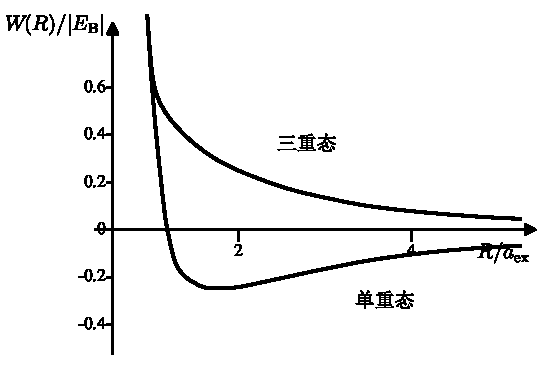
\includegraphics[width=6.5cm]{fig10-4.pdf}\\[0.2em]
{\small 图 10.4\quad $m_{\mathrm{h}}^{*}\gg m_{\mathrm{e}}^{*}$ 极限的双激子的互作用}\\[0.2em]
{\small （$|E_{\mathrm{B}}|\equiv e^{2}/(2\epsilon a_{\mathrm{ex}})$ 为瓦尼尔-莫特激子的结合能）}
\end{minipage}
\end{center}

双激子分子的基态波函数按海特勒-伦敦近似写为
\begin{equation}
\begin{aligned}
  \varPhi_{\mathrm{H}-\mathrm{L}}
  &=C_{\mathrm{s}}\left[\varphi_{\mathrm{a}}(1)\varphi_{\mathrm{b}}(2)
  +\varphi_{\mathrm{b}}(1)\varphi_{\mathrm{a}}(2)\right]\\
  &\quad\times\frac{1}{\sqrt{2}}\left[\chi_{\uparrow}(1)\chi_{\downarrow}(2)
  -\chi_{\downarrow}(1)\chi_{\uparrow}(2)\right]
\end{aligned}
\end{equation}
其中 $\chi_{\sigma}\left(\sigma=\uparrow,\downarrow\right)$ 代表自旋朝上和朝下态，而
\begin{equation}
  \varphi_{\mathrm{a}}(1)\equiv\pi^{-\frac{1}{2}}\exp\left(-r_{1\mathrm{a}}\right)
  \text{，}\qquad
  \varphi_{\mathrm{b}}(2)\equiv\pi^{-\frac{1}{2}}\exp\left(-r_{2\mathrm{b}}\right)
\end{equation}
是1s态激子的相对运动波函数，其中 $r_{1\mathrm{a}}$，$r_{2\mathrm{b}}$，…是以激子半径 $a_{\mathrm{ex}}$ 为单位的相对坐标.这样，在 $\sigma=0$ 极限双激子分子基态波函数的空间部分可写为
\begin{equation}
\begin{aligned}
  \psi_{\mathrm{H}-\mathrm{L}}&=(2C_{\mathrm{s}}/\pi)
  \exp\left[-(1/2)\left(r_{1\mathrm{a}}+r_{1\mathrm{b}}+r_{2\mathrm{a}}+r_{2\mathrm{b}}\right)\right]\\
  &\quad\times\cosh\left[-(1/2)\left(r_{1\mathrm{a}}-r_{1\mathrm{b}}-r_{2\mathrm{a}}+r_{2\mathrm{b}}\right)\right]
\end{aligned}
\end{equation}
上式中归一化参数 $C_{\mathrm{s}}$ 是R的函数.

\subsection*{(ii) $\sigma=1$ 极限}

这时 $m_{\mathrm{e}}^{*}=m_{\mathrm{h}}^{*}$，和氢分子问题差别很大，但与正电子素分子(positronium molecule)问题相似.惠勒(Wheeler)指出\textsuperscript{[6]}，用H-L型波函数不能求得两个正电子和两个负电子的束缚态(即正电子素分子).海勒拉斯(Hylleraas)和奥雷(Ore)引入下列试探函数\textsuperscript{[7]}（以下简称H-O函数）
\begin{equation}
\begin{aligned}
  \psi_{\mathrm{H}-\mathrm{O}}&=2\exp\left[-(1/2)\alpha
  \left(r_{1\mathrm{a}}+r_{1\mathrm{b}}+r_{2\mathrm{a}}+r_{2\mathrm{b}}\right)\right]\\
  &\quad\times\cosh\left[-(1/2)\beta\alpha
  \left(r_{1\mathrm{a}}-r_{1\mathrm{b}}-r_{2\mathrm{a}}+r_{2\mathrm{b}}\right)\right]
\end{aligned}
\end{equation}
其中 $\alpha$、$\beta$ 为可调参数，他们利用变分法算得了正电子素分子的结合能.沙尔玛(Sharma)\textsuperscript{[8]}将H-O函数用于双激子分子，证明了在 $\sigma=m_{\mathrm{e}}^{*}/m_{\mathrm{h}}^{*}=1$ 极限下也有稳定的分子结合，$\sigma=1$ 情况又称为正电子素分子极限.

\subsection*{(iii) $0<\sigma<1$ 情况}

作为一般情况的讨论，只需要研究 $\sigma$ 在0与1之间系统的性质，因为由于对称性 $\sigma>1$ 区域与 $\sigma<1$ 区是等效的，可以从 $\sigma<1$ 推知 $\sigma>1$ 情况，由此可得任意 $\sigma$ 比值的信息.阿达莫夫斯基(Adamowski)等\textsuperscript{[9]}仅仅从哈密顿量的结构就证明了 $0\leqslant\sigma\leqslant1$ 范围内激子分子的结合能与激子结合能之比只是 $\sigma$ 的单调衰减函数.因此，如果在 $\sigma=1$ 极限情况下证明了双激子分子的结合，则在 $0<\sigma<1$ 区域（以致全 $\sigma$ 区）内激子分子将是稳定的.从物理角度分析，阿达莫夫斯基的结论也是合理的.当 $\sigma$ 从零开始增大时，主要差别仅在于使空穴局域化必须增大动能，它随着 $\sigma$ 单调增加，从而降低结合能，到达 $\sigma=1$ 时结合能下降到最低值.对于 $\sigma>1$ 情况，可以将空穴当作“轻粒子”，电子当作“重粒子”重新定义 $\sigma$，作相似的讨论.

在这个区域中激子分子的结合能的定量计算主要由花村(Hanamura)\textsuperscript{[3]}和莱斯(Rice)\textsuperscript{[4]}两个小组作出，他们将H-O函数推广为
\begin{equation}
  \psi=f(R)g\left(\xi_{1},\eta_{1},\xi_{2},\eta_{2};R\right)
\end{equation}
这里
\begin{equation}
  f(R)=R^{\gamma/2}\exp\left(-\delta R/2\right)
\end{equation}
$g$ 就是 $\psi_{\mathrm{H}-\mathrm{O}}$ 的另一写法
\begin{equation}
  g=\exp\left[-(1/2)\alpha\left(\xi_{1}+\xi_{2}\right)R\right]
  \times\cosh\left[(1/2)\beta\alpha\left(\eta_{1}-\eta_{2}\right)R\right]
\end{equation}
$\alpha$、$\beta$、$\gamma$、$\delta$ 为独立变分参数，$\xi_{i}$ 和 $\eta_{i}\ (i=1,2)$ 由下列关系定义
\begin{equation}
  \xi_{i}=\left(r_{i\mathrm{a}}+r_{i\mathrm{b}}\right)/R
  \text{，}\qquad
  \eta_{i}=\left(r_{i\mathrm{a}}-r_{i\mathrm{b}}\right)/R
\end{equation}
这样写，是为了计算时便于运用旋转椭球坐标.当参数 $\gamma$ 和 $\delta$ 都趋向无穷大，且有固定比值 $(\gamma/\delta)=R_{0}$ 时，式(10.5.7)具有 $\delta\left(R-R_{0}\right)$ 函数特征，若再设 $\alpha=1$ 和 $\beta=-1$，则式(10.5.8)简化为(10.5.4)，这时 $\varPsi$ 代表固定 $R=R_{0}$ 值时的H-L近似波函数，可描述氢分子极限.如果令 $\gamma=\delta=0$，则 $f(R)=1$，$\varPsi=\psi_{\mathrm{H}-\mathrm{O}}$ 代表正电子素分子极限.这说明选择式(10.5.6)—(10.5.8)作为试探波函数是合理的.他们计算的结果由图10.5表示，正如阿达莫夫斯基所预料，激子分子的结合能与激子结合能的比值 $|E_{\mathrm{M}}|/|E_{\mathrm{B}}|$ 是 $\sigma$ 的单调衰减函数.

以上结果说明，对于电子和空穴有效质量比的任意值，双激子分子均是稳定的.同时，实验上也已证实在一系列半导体（如CuCl、CuBr、CdS、CdSe等)中均存在双激子分子.

双激子具有类玻色子特征，又由于它的平移质量很轻，因此双激子系统的量子效应可能比液氦更为显著.有许多理论工作者曾预言有双激子系统的玻色凝聚\textsuperscript{[3]}，但至今尚无确切的实验证明.

\begin{center}
\begin{minipage}{5.5cm}
\centering
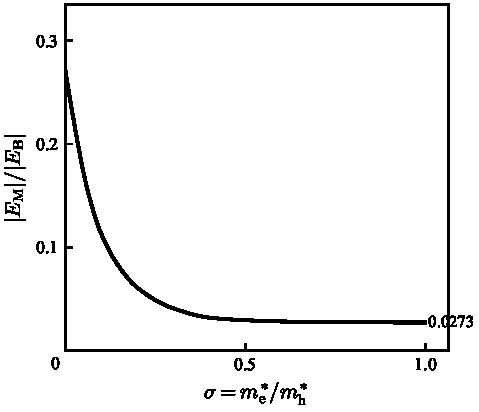
\includegraphics[width=5.5cm]{fig10-5.pdf}\\{\small 图 10.5\quad 激子分子结合能与 $\sigma$ 的关系}
\end{minipage}
\end{center}

\subsection*{2. 电子-空穴液体}

为了研究激子系统的相变，必须在本征半导体中产生高浓度的电子-空穴对激发.近年来利用皮秒激光(picosecond laser)技术，在非直接能隙半导体(如Ge、Si)中可以产生任意高浓度的激发，并观测到电子-空穴液滴.

从能带论角度讲，半导体可分为两类：一类是导带极小和价带极大（带边）具有相同的波矢值，称为直接能隙半导体，InSb、InAs、GaAs等属于这一类，它们的导带和价带边都在 $\boldsymbol{k}=0$ 处（Γ点）.另一类半导体其导带极小与价带极大的 $\boldsymbol{k}$ 值位于BZ中不同点，称为非直接能隙半导体，Ge、Si等属于非直接能隙半导体.在Ge晶体中价带边位于 $\boldsymbol{k}=0$（Γ点），但导带边在[111]方向的BZ边界的L点上 $\boldsymbol{k}=\frac{2\pi}{a}\left(\frac{1}{2},\frac{1}{2},\frac{1}{2}\right)$ 处，导带有4个等效的电子能量极小点，对应于四重简并，在极值附近的等能面是以[111]为轴的旋转椭球，平行和垂直转轴的有效质量分别为 $m_{\mathrm{eL}}^{*}=1.59m_{\mathrm{e}}$，和 $m_{\mathrm{eT}}^{*}=0.082m_{\mathrm{e}}$.Si的价带边也在Γ点，但导带边位于[100]方向上 $\frac{2\pi}{a}(0.86,0,0)$ 处（在BZ中Δ轴上靠近H点），等能面是以[100]为轴的旋转椭球，$m_{\mathrm{eL}}^{*}=0.92m_{\mathrm{e}}$，$m_{\mathrm{eT}}^{*}=0.19m_{\mathrm{e}}$，BZ内有6个等效的电子能量极小点，对应于六重简并，它们的能带曲线可参考文献\textsuperscript{[10]}.

在非直接能隙半导体中，因辐照激发的非平衡载流子(电子和空穴)将立刻弛豫到能带的极值处，库仑作用使它们形成激子，其中电子与空穴的波矢值不相同，这一特点要求非直接能隙半导体中激子的复合辐射必须有声子参加，否则就不能保持动量守恒.由于这个缘故，Ge和Si中激子的寿命可长达微秒量级，比非平衡载流子过渡到热平衡分布所需的时间(纳秒)长得多.所以，利用Ge、Si为背景材料，可以产生高浓度的、处于准平衡状态的激子系统，为激子相变的实验研究提供了条件.

只有在低浓度条件下，电子-空穴系统才可以看作是激子气体，在高浓度极限时，激子间的重叠十分强烈，以致使激子失去了它的个别特性，激子将离子化而不再作为一个确定的实体存在.1968年凯尔狄希(Keldysh)在第九届国际半导体会议上首先指出：高浓度条件下电子-空穴系统的最稳相可能是金属性的电子-空穴液体，这是由电子和空穴组成的二分量费密液体，简称为E-H液体.从此，理论工作者面临着一个课题，必须计算E-H液体中平均每个电子-空穴对的基态能量 $E_{\mathrm{G}}$，只有当 $|E_{\mathrm{G}}|$ 大于单激子结合能时，才能说明E-H液体是系统的稳定相.从多体理论角度讲，E-H液体的基态能由3部分组成：(i)电子系统和空穴系统的动能 $E_{\mathrm{K}}$，(ii)电子间和空穴间的交换能 $E_{\mathrm{ex}}$，(iii)相关能 $E_{\mathrm{corr}}$.为简便起见，先看各向同性非简并能带模型的计算结果；对于这种理想化的能带模型，电子与空穴的等能面都呈球形，因此依照电子体系理论［见式(4.9.14)］容易求得E-H液体中平均每个电子-空穴对的动能和交换能为
\begin{equation}
  E_{\mathrm{K}}=\frac{3}{5}\biggl(\frac{\hbar^{2}k_{\mathrm{F}}^{2}}{2m_{\mathrm{e}}^{*}}
  +\frac{\hbar^{2}k_{\mathrm{F}}^{2}}{2m_{\mathrm{h}}^{*}}\biggr)
  =\frac{3}{5}\frac{\hbar^{2}k_{\mathrm{F}}^{2}}{2\overline{M}}
  =\frac{2.21}{r_{\mathrm{s}}^{2}}\ [\text{激子 Ry}]
\end{equation}
\begin{equation}
  E_{\mathrm{ex}}=-\frac{3e^{2}k_{\mathrm{F}}}{2\pi}
  =-\frac{1.832}{r_{\mathrm{s}}}\ [\text{激子 Ry}]
\end{equation}
其中 $k_{\mathrm{F}}$ 为费密波矢，$\overline{M}$ 是电子-空穴对的折合质量.$r_{\mathrm{s}}$ 代表以激子半径 $a_{\mathrm{ex}}=\epsilon\hbar^{2}/(\overline{M}e^{2})$ 为单位的平均电子(或空穴)间距，它是和电子-空穴对浓度n有关的参数
\begin{equation}
  n=\frac{3}{4\pi r_{\mathrm{s}}^{3}a_{\mathrm{ex}}^{3}}
\end{equation}
式(10.5.10)和(10.5.11)的最后等式以单激子结合能 $|E_{\mathrm{B}}|=e^{2}/(2\epsilon a_{\mathrm{ex}})$ 为单位，称为激子的里德伯单位.对于相关能，花村\textsuperscript{[11]}用高密度展开法作了初步估计，当 $\sigma=1$ 时得到
\begin{equation}
  E_{\mathrm{corr}}=0.497\ln r_{\mathrm{s}}-0.33\ [\text{激子 Ry}]
\end{equation}
代入基态能公式，
\begin{equation}
\begin{aligned}
  E_{\mathrm{G}}\left(r_{\mathrm{s}}\right)&=E_{\mathrm{K}}+E_{\mathrm{ex}}+E_{\mathrm{corr}}\\
  &=2.21/r_{\mathrm{s}}^{2}-1.832/r_{\mathrm{s}}+0.497\ln r_{\mathrm{s}}-0.33\ [\text{激子 Ry}]
\end{aligned}
\end{equation}
根据上式所作能量-密度曲线的极小值在 $r_{\mathrm{s}}=1.7$ 处，对应的能量极值为 $E_{\mathrm{G}}=-0.38$.显然这个数值比单个激子的基态能 $-1$ 高得多，不能说明E-H液体是稳定相.随后有一系列工作严格计算相关能，所得的 $E_{\mathrm{G}}\left(r_{\mathrm{s}}\right)$ 曲线如图10.6中虚线所示，对于各向同性非简并能带模型的极小点在 $r_{\mathrm{s}}=1.95$ 处，$E_{\mathrm{G}}=-0.86$，仍然高于 $-1$，迄今最好的多体计算也不能证明 $E_{\mathrm{G}}<-1$\textsuperscript{[4]}.莱斯\textsuperscript{[12]}和诺齐尔斯(Nozieres)\textsuperscript{[13]}两个小组同时指出：必须考虑Ge、Si能带的简并和各向异性结构才能算得 $E_{\mathrm{G}}<-1$，从而证明了E-H液体是高浓度时系统的稳定相.他们计算的动能和交换能有解析表示，在激子里德伯单位中可写成：
\begin{equation}
  E_{\mathrm{K}}=\frac{0.468}{r_{\mathrm{s}}^{2}}\text{，}\quad
  E_{\mathrm{ex}}=-\frac{1.136}{r_{\mathrm{s}}}\ (\mathrm{Ge})
\end{equation}
\begin{equation}
  E_{\mathrm{K}}=\frac{0.727}{r_{\mathrm{s}}^{2}}\text{，}\quad
  E_{\mathrm{ex}}=-\frac{1.157}{r_{\mathrm{s}}}\ (\mathrm{Si})
\end{equation}
但是相关能只有数值结果.对于Ge，$E_{\mathrm{G}}\left(r_{\mathrm{s}}\right)$ 曲线由图10.6中实线表示，其极小点在 $r_{\mathrm{s}}=0.63$ 处，极小点能量 $E_{\mathrm{G}}=-2.0$ 与 $r_{\mathrm{s}}$ 相应的电子-空穴对浓度 $n_{0}\approx2\times10^{17}\ \mathrm{cm}^{-3}$，用通常单位表示的 $|E_{\mathrm{G}}|=5.3$ meV，这个数值比Ge中激子结合能 $|E_{\mathrm{B}}|=4.15$ meV大得多，说明在高浓度条件下Ge中E-H液体是系统的基态，对于Si也有相似的结果.将式(10.5.10)与（10.5.11）和式（10.5.15）与(10.5.16)相比较，可以看出能带的简并和各向异性所引起系统动能的减少比交换能的减少大得多，这有利于E-H液体的能量降低.

\begin{center}
\begin{minipage}{6.5cm}
\centering
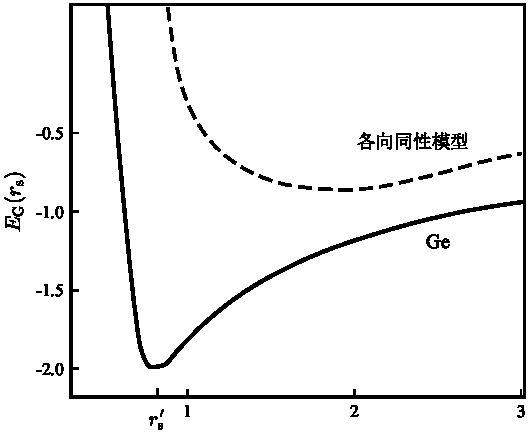
\includegraphics[width=6.5cm]{fig10-6.pdf}\\{\small 图 10.6\quad E-H液体的基态能的计算曲线\textsuperscript{[12,13]}}
\end{minipage}
\end{center}

在有限温度，当电子-空穴对的平均浓度小于 $n_{0}$ 时，E-H液体中将分离出低浓度的气相(激子气体)，并形成E-H液体和激子气体的两相共存区.这时，实验上就能观测到电子-空穴液滴.近年来，对于E-H液体的相图，应力、磁场等外界条件对E-H液体的影响，以及电子-空穴液滴的生长等问题都进行了系统研究\textsuperscript{[4,5]}.高密度条件下激子系统的相变问题已成为固体理论研究的新领域.

\begin{canKao}
\begin{enumerate}[label={[\arabic*]}, leftmargin=2.2em, itemsep=0pt]
\item Gross E F et al. Dokl Akad Nauk SSSR, 1953, 92: 265
\item Nakajima S et al. The Physics of Elementary Excitations. New York: Springer-Verlag, 1980. Chap 2
\item Hanamura E, Haug H. Phys Rep, 1977, 33C: 209
\item Rice T M. Solid State Phys, 1977, 32: 1
\item Hensel J C et al. Solid State Phys, 1977, 32: 88
\item Wheeler J A. Ann New York Acad Sci, 1946, 48: 219
\item Hylleraas E A, Ore A. Phys Rev, 1947, 71: 493, 913
\item Sharma R R. Phys Rev, 1968, 170: 770; 1968, 177: 36
\item Adamowski J A et al. Solid State Commun, 1971, 9: 2037; Phil Mag, 1972, 26: 143
\item Kittel C. Introduction to Solid State Physics. New York: Wiley, 1976. Chap 8
\item Hanamura E. Proc Int Conf Phys Semicond 10th. Virgina: Spring-field, 1970. 351
\item Brinkmann W F, Rice T M, Anderson P W, Chui S T. Phys Rev Lett, 1976, 28: 961; Phys Rev, 1973, B7: 1508
\item Combescot M, Nozieres P. J Phys, 1972, C5: 2369
\end{enumerate}
\end{canKao}
